\section{Aplicação móvel}
A versão móvel da aplicação contém cinco páginas: introdutória, nova música, interpretação, playSong e About Us.

\subsection{Página Introdutória}
Nesta página (ver \autoref{intro}) faz-se uma introdução da aplicação móvel com uma ligação para entrar na página "nova música". Esta página é a única que não contém as barras fixas superior e inferior de navegação: na superior encontra-se o nome da página actual e um botão para regressar à pagina introdutória com atualização da aplicação móvel (lado direito). Finalmente, na barra inferior, temos disponíveis a ligações de interesse para as restantes páginas da aplicação móvel. (ver \autoref{music}, \autoref{inter}, \autoref{play} e \autoref{us}).

\begin{figure}[htp]
\centering
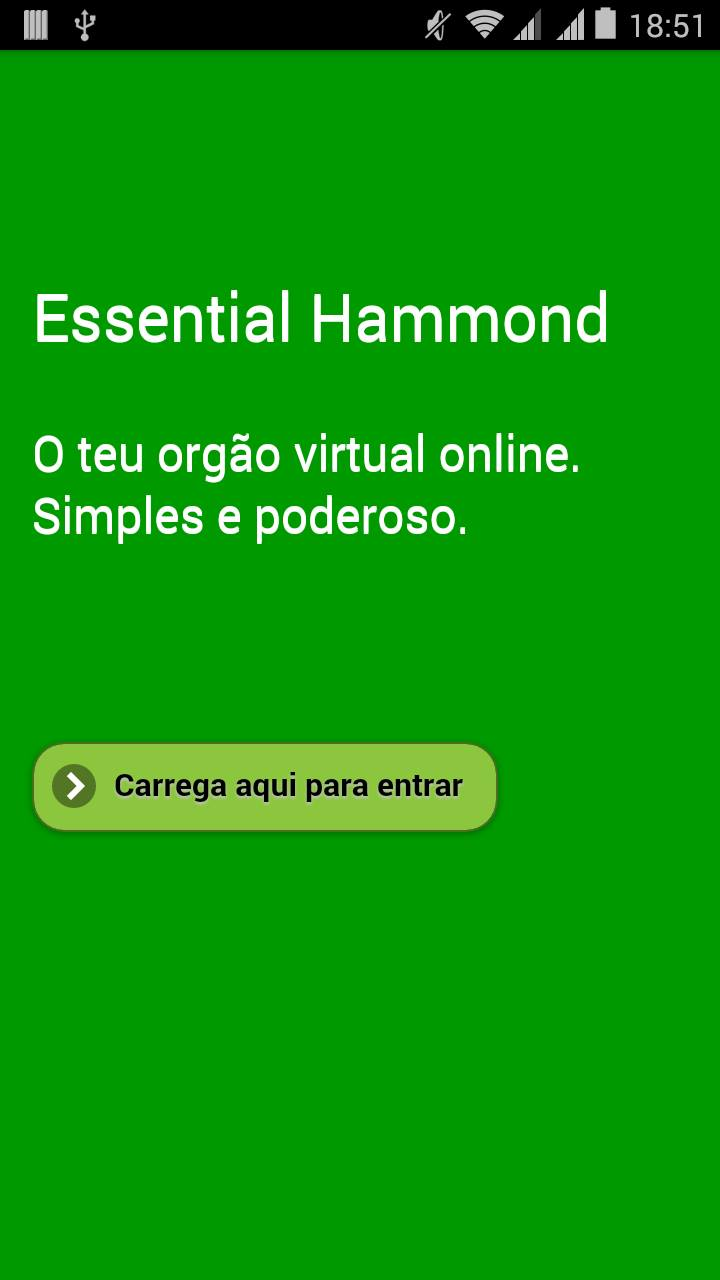
\includegraphics[width=50mm]{images/appIntro.jpg}
\caption{Página Introdutória da aplicação móvel.}
\label{intro}
\end{figure}

\subsection{Nova Música}
Nesta secção, o utilizador pode escrever as suas pautas na caixa de texto criada para o efeito e enviar para o servidor através de um botão (ver \autoref{music}). Quando o processamento é finalizado é enviado uma mensagem ao utilizador de acordo com o sucesso ou o insucesso do mesmo. 

\begin{figure}[htp]
\centering
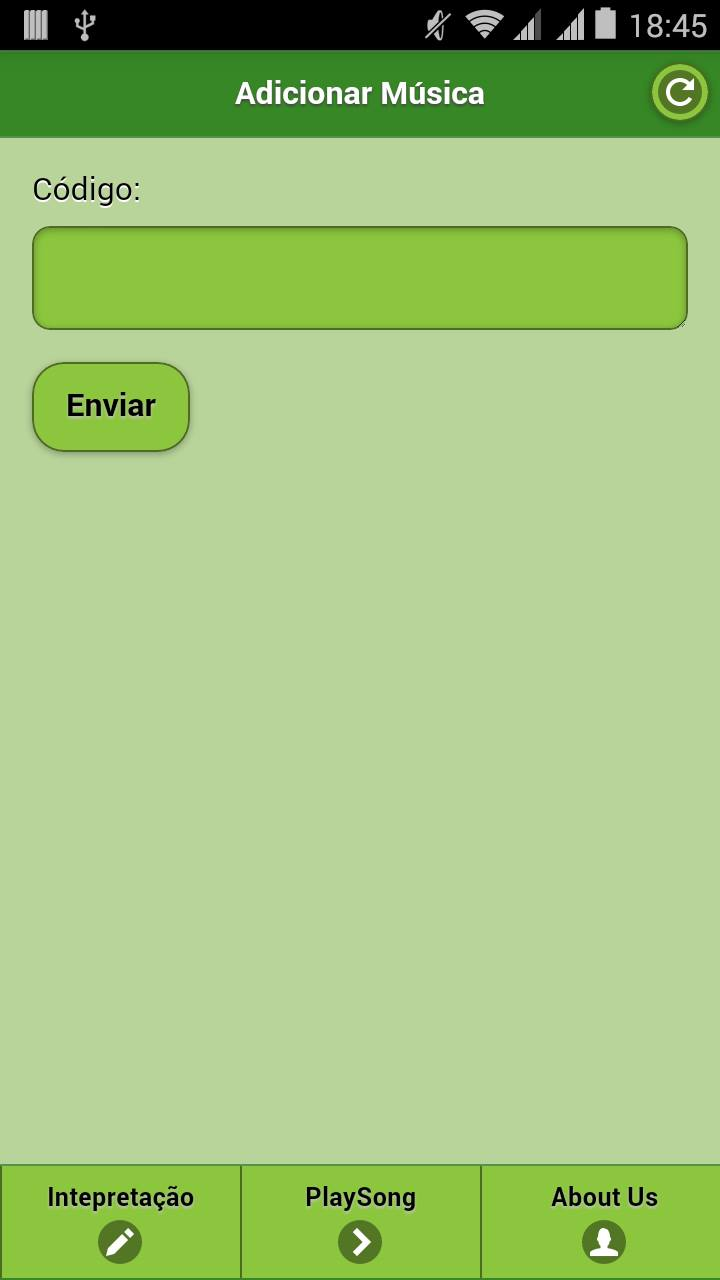
\includegraphics[width=50mm]{images/appAddNote.jpg}
\caption{Página de envio da música ao servidor.}
\label{music}
\end{figure}

\subsection{Interpertação}
Esta página corresponde ao último passo que o utilizador tem de dar para a criação do ficheiro audio. Para isso, ele tem de escolher a música, registo, efeito e o nome para o ficheiro, como podemos ver na figura \autoref{inter}. Como na página "Nova Música", o utilizador vai receber mensagens de aviso após o processamento do servidor.

\begin{figure}[htp]
\centering
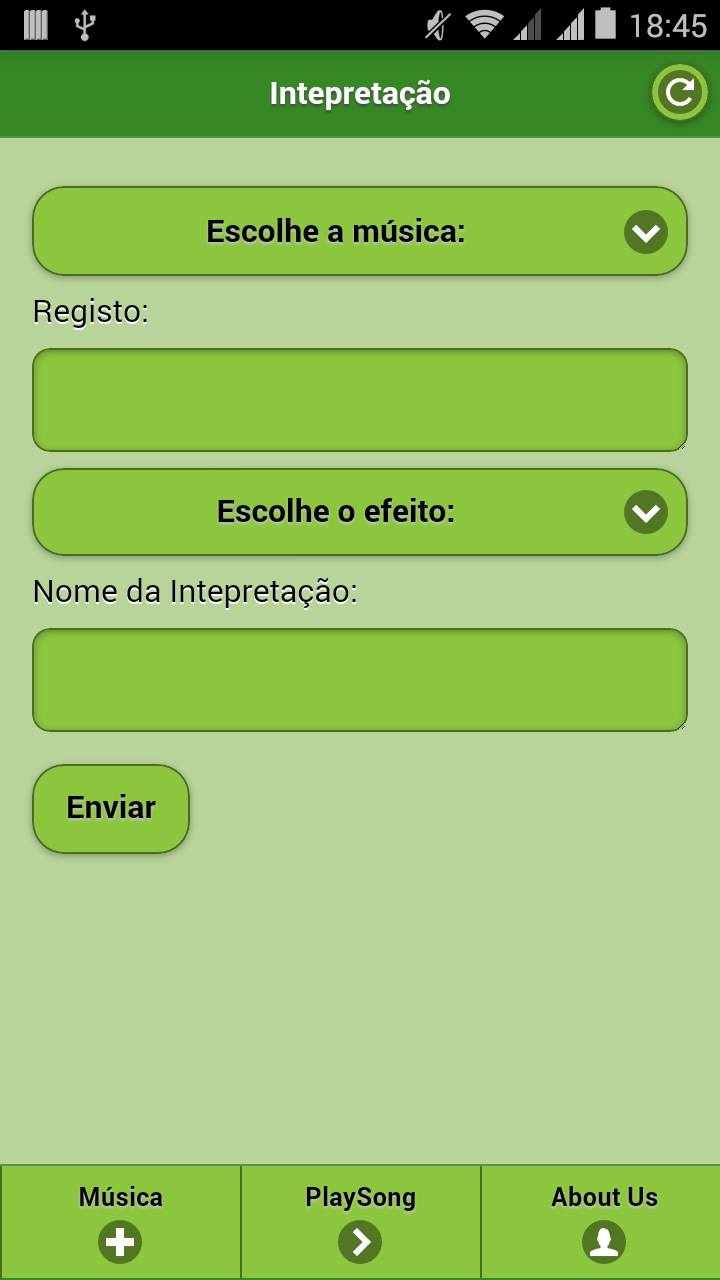
\includegraphics[width=50mm]{images/appAddMusic.jpg}
\caption{Página de envio da interpretação ao servidor.}
\label{inter}
\end{figure}

\subsection{PlaySong}

Inicialmente, nesta página, o utilizador tem disponível um \emph{pop-up} para escolher a música. Ao pressionar no botão "Procurar", a app móvel irá encontrar as interpretações que a musica anteriormente escolhida está associada e serão imediatamente visiveis. Cada interpretação irá conter um \emph{slidedown} individual com várias funcionalidades: contagem de gostos e não gostos, botões de gosto e não gosto, um botão "imagem" em que a imagem da pauta será visualizada através de um \emph{pop-up} e, finalmente, a reprodução audio da interpretação em questão (ver figura \autoref{play}).

\begin{figure}[htp]
\centering
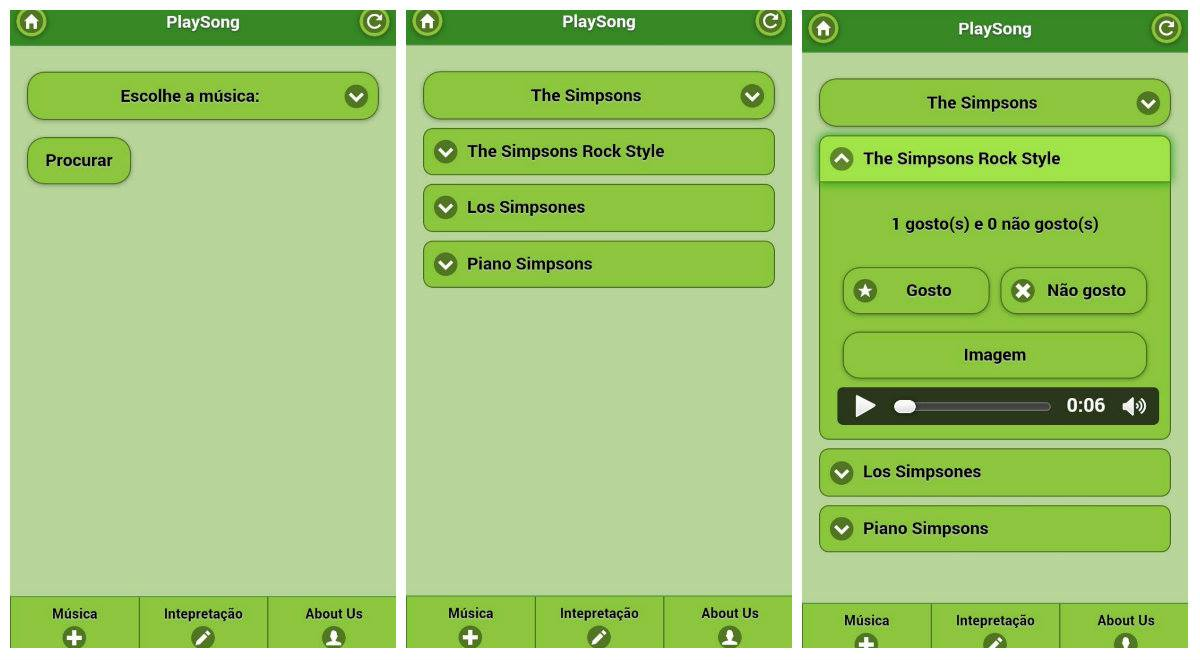
\includegraphics[width=\textwidth]{images/appPlaySong.jpg}
\caption{Página de reprodução das interpretações e mais algumas funcionalidades.}
\label{play}
\end{figure}

\subsection{About Us}

Nesta página, serão visualizados todos os alunos responsáveis pela a criação desta aplicação. Ao carregar num aluno abre-se um \emph{pop-up} contendo mais informações sobre o aluno, como a cidade, idade, curso e nº mecanográfico. (ver figura \autoref{us}).

\begin{figure}[htp]
\centering
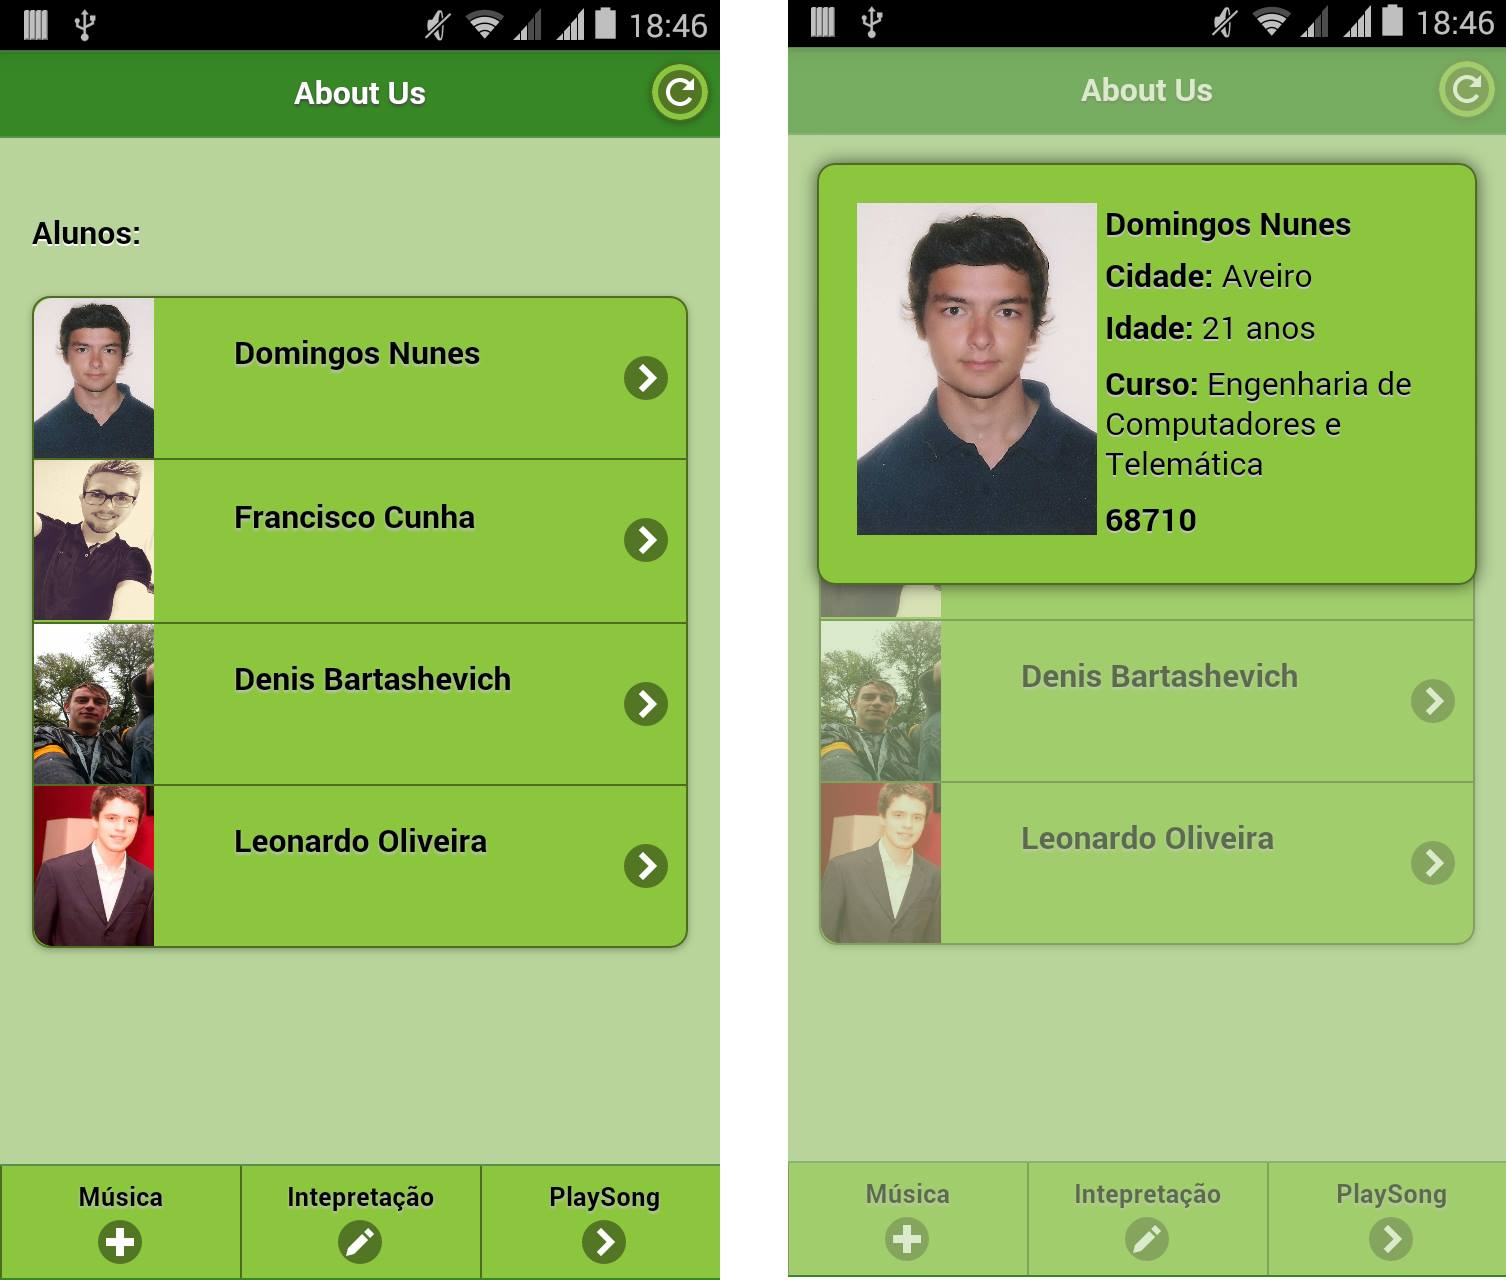
\includegraphics[width=\textwidth]{images/appUs.jpg}
\caption{Página sobre o grupo responsável por este trabalho.}
\label{us}
\end{figure}